\chapter{Introduction}
\label{cha:intro}
In this chapter we begin by outlining the justifications behind our research into this field, highlighting the absence of current work accounting for stochastic routing in the field of network tomography in \cref{sec:Imotivationandoutline}. We then identify specific sub-problems within the existing work on stochastic routing and pose solutions to these problems
in the form of project wide scope goals.\par
Next an overview of current models and inferential techniques used in stochastic network tomography is provided in \cref{sec:Imodels}. We these models into their three major components: network generation, traffic simulation, and inferential calculations.\par
We then present new metrics used within our tomographic method and alternative fixed probe packet routing methods. A summary of introduced concepts and information is then provided in \cref{sec:Iintroductionsummary}.\par

\section{Outline and Motivation}
\label{sec:Imotivationandoutline}

Network tomography is the technique of using end-to-end measures to make inferences about a computer network. In this way it is similar to computed axial tomography (CAT) scans in the medical world - a process whereby x-rays are passed through a patient as a noninvasive means of gaining information pertaining to the patient's interior. These x-rays are fired from multiple points around the patient's exterior. They attenuate as they pass through different densities of tissue and are measured as they exit the body. This process results in the calculation of a single two-dimensional slice of the body's tissue density. This is typically repeated over many adjacent slices to give a 3-dimensional representation.\par
Network tomography is most analogous to a single CAT slice. However instead of using the attenuation of x-rays to infer body tissue density we send network packets on predefined routes between observable \textit{monitor nodes} and measure the latency of communication. This allows us to infer the structure and behaviour of routers within a network. A high level illustration of the problem is given in \ref{fig:nettom?}.\par
In network science this latency is referred to as a delay and is calculated as the time a given \textit{packet} or discrete signal takes to traverse the network to its predetermined destination. In network science there are various forms of signal casting - primarily broadcasting, uni-casting, multi-casting, and any-casting- we will focus on the case of a uni-casted signal, as the inclusion of alternative casting methods would introduce too great a complexity for one study. We note that sub-fields of research already exist for tomography under each casting method(\cite{lawrence_network_2006}).\par
\begin{figure}
    \centering
    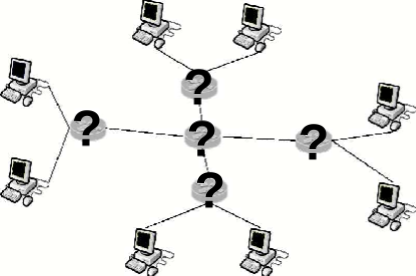
\includegraphics[width=10cm]{figs/intro/nettom-illustration.png}
    \caption[Illustrative example of network requiring tomographic probing]{Illustrative example of network requiring tomographic probing (\cite{lawrence_network_2006})}
    \label{fig:nettom?}
\end{figure}

Network tomography is primarily used for: topology identification (\cite{zhang_topology_2014}, \cite{hailiang_network_2009}), general internal state inference (\cite{vardi_network_1996}, \cite{coates_network_2001}, \cite{he_network_2021}) and, in the case of Boolean tomography, node failure localisation (\cite{nguyen_boolean_2007}, \cite{ma_optimal_2015}). In this thesis we focus on internal state inference; specifically, in the identification of abnormal behaviour of network components as potentially caused by an attacker intent on disrupting network behaviour. We refer to these induced cases of abnormal behaviour, and the offending network components causing these, as \textit{nefarious}.\par
As network tomography is advances as a discipline, it is beginning to be implemented in many real-world settings. It is now supported by emerging platforms such as Consul (\cite{shilton_network_2021}) and will see support in future network coding approaches, as discussed in \cite{kakkavas_review_2020}. The increasing use of network tomography in real-world settings therefore demands research into methods of further validating and optimising the performance of network tomography in industrial-, public- and private-communication infrastructure settings.\par
Historical work on uni-cast tomography has focused primarily on networks with an absence of queue buffers (this absence resulting in packets taking static paths through a network). \cite{lai_measuring_2000} expanded this focus by investigating routing behaviours present in stochastically routing networks. Recent work by \cite{barnes_stochastic_2020} has used the approach of \cite{lai_measuring_2000} to introduce nefarious behavior in stochastic settings and subsequently to detect such behaviours. In doing this Barnes developed a simulation more applicable to real world networks.\par
We aim to build upon this work of nefarious behaviour detection in stochastic environments. To do so, we will relax further assumptions to better simulate mid-sized complex real world networks such as a home or IoT network. We focus on ensuring that methods employed are scalable to far larger networks. In doing so, we hope to establish that the approach is generally applicable to large-scale real-world networking such as those seen in the academic, consumer ISP and commercial data center networks that underpin modern cloud infrastructure. The key assumptions upon which Barnes based their work are:\par
\begin{enumerate}
\item \emph{All packets originate and terminate at switches.}
\item \emph{All routers which are not nefarious behave identically.}
\item \emph{Packets are not dropped when traffic is heavy, instead accumulating in queues of unbound length.}
\item \emph{All end nodes are equally likely to send packets, and be chosen to receive packets.}
\item \emph{All routing protocols are the same for non-nefarious routers.}
\item \emph{Background traffic across the network has a constant average intensity.}
\item \emph{End Nodes of the network are switches.}
\item \emph{The service time for every packet at the front of the queue in a router is 1 “time step”.}
\end{enumerate}

We focus on the relaxation of assumptions 1-5, and leave future work to address additional assumptions. We choose not to relax assumption 6 as it allows for a bounded network size. Without switches as end nodes we would be forced to instead recursively model all connected sub-networks. This would eventually lead to a model that represented the entire observable internet connected to this network; being unbounded in size, this would be both impractical and of little use to analyse. Maintaining assumption 1 allows for analysis of arbitrary sub-networks that may be of interest to the typical network administrator. Adjacent networks can be represented as single node with a number of switches connected proportional to the typical traffic from that network.We chose not to relax assumption 8, as it is key to the analysis technique used within our work. The difficulty behind its relaxation is expanded in \cref{sec:Rnefarouterdetection}, and the relaxation of this particular assumption is left to further work on the topic.\par
In relaxing these assumptions and implementing extensions, we hypothesise that network tomography can be used to estimate routers' buffer queue lengths with sufficient accuracy to enable inference of packet delaying behaviour by individual routers within real world networks. Due to the large scope of this hypothesis, we decompose it into 2 sub-hypothesis:
\begin{enumerate}
    \item Network tomography enables inference of node level packet delay metrics within stochastically routing real-world networks.
    \item A router can be classified as exhibiting nefarious behaviour or not using information gained from packet delay metrics.
\end{enumerate}
As real-world use of network tomography is exponentially more complex than previous mathematical models, in tackling sub-hypothesis 1 we introduce an alternative and novel method of packet delay average (PDA) tomography (\cref{sssec:Iinferentialcalculations}). To evaluate sub-hypothesis 2, we perform a series of experiments that vary network parameters (\cref{sec:MNefidentification}). From these we develop three binary classifiers to identify nefarious routers under three sets of assumptions. We evaluate each of these classifiers against the requirements of three real-world use cases.\par
Compared to previous theoretical methods, our approach classifies nefarious nodes less accurately and less precisely. However, we utilise optimization techniques (presented in \cref{sec:Boptimization}) to maximise the accuracy of our novel methods. To measure the impact of optimisations, we quantify the maximum potential accuracy of our inferences using statistical methods from link-focused tomography, as outlined in \cite{he_fisher_2015}. We represent all known information about the network using its Fisher information (see \cref{ssec:Bfisherinformation}). This representation results in the maximum potential accuracy of our analysis being given by the Cramér–Rao Bound (see \cref{ssec:Bcrb}).\par
Additionally we hope this work on the power of tomography in an adversarial setting will spur interest in the fledgling field of adversarial tomography. We note that few studies on the topic have been conducted to date (\cite{he_network_2021}) and believe further research in this area could be extremely beneficial to the security and networking communities.

\section{Stochastic Network Tomographic Models}
\label{sec:Imodels}

In this section we introduce existing models and methods for stochastic network tomography in literature. For ease of discussion, we split these models into three sections: network generation, traffic simulation and inferential calculations. This decomposition was chosen as each section can be treated as a distinct process, with the output from each able to be parsed to the next in a context-free manner. In \cref{ssec:Icurrentmodels} we cover specific methods currently used for each of these three areas. In \cref{sssec:Itrafficsimulation} we narrow our focus to traffic and delay simulation, highlighting assumptions and key segments for potential improvement in current models. Finally we provide an overview of the model produced as a key deliverable of this project, outlining differences from the current work.

\subsection{Previous Models}
\label{ssec:Icurrentmodels}

Previous work surrounding network tomographic models identifying nefarious nodes in stochastic networks is led by \cite{barnes_stochastic_2020}. This work takes a theoretical mathematical approach to tomography, and was based upon the requirement that the system be described by a formal mathematical model. In this section we introduce approaches used in Barnes's work along with candidate areas considered for extension. We provide additional explanation and background of these techniques in \cref{cha:background}. We note that work in both \cite{he_fisher_2015} and \cite{kolar_distributed_2020} also covers stochastic environments. Both these studies, however, focus on link level metrics. Notwithstanding this, in  \cref{ssec:Idevelopedmodels} we show how techniques from previous work on link metrics can be adapted for use in our setting.

\subsubsection*{Network Generation}
\label{sssec:Inetworkgeneration}

The goal of network generation in the context of validating tomographic models is the production of a random undirected graph representing a small to medium sized network. The generated network must contain four essential components: 
\begin{enumerate}
    \item \textit{Routers} to direct packets.
    \item \textit{Switches} to emulate connection to a larger external network (i.e. the world wide web) through stochastic production of packets (elaborated upon in \cref{sssec:Itrafficsimulation}).
    \item \textit{Monitors} which we are particular switches we are able to directly control and observe.
    \item \textit{Links} between routers for packets to traverse.
\end{enumerate}
Components 1, 2, and 3 are represented as nodes within the graph, and component 4 is represented by edges between nodes. The generation of these pseudo-random networks is desirable for verification of tomographic techniques in a controlled environment as it allows for many topologies to be tested, thereby ensuring the robustness of introduced techniques.\par
Previous work around nefarious router identification in stochastic networks (by \cite{barnes_stochastic_2020}) employs a user-defined connectivity parameter to generate edges between nodes. This is analogous to the Erdos-Renyi (ER) generation technique originally posed in \cite{erdos_random_1959}. We provide formal definitions of this technique in \cref{sec:Bgraphgeneration}. In real-world networks, however, router degree (the number of connected routers and switches) converges to a power law (\cite{chen_origin_2002}, \cite{zhao_measurement_2020}). Such graphs are commonly referred to as scale-free. In contrast to this, a Poisson distribution of node degree is observed in other, more naive, network generation algorithms such as the Erdős–Rényi model. A comparison of node degree between graphs generated with an ER technique and those generated with a scale free technique is given in \ref{fig:nddist}.\par
\begin{figure}[t]
    \centering
    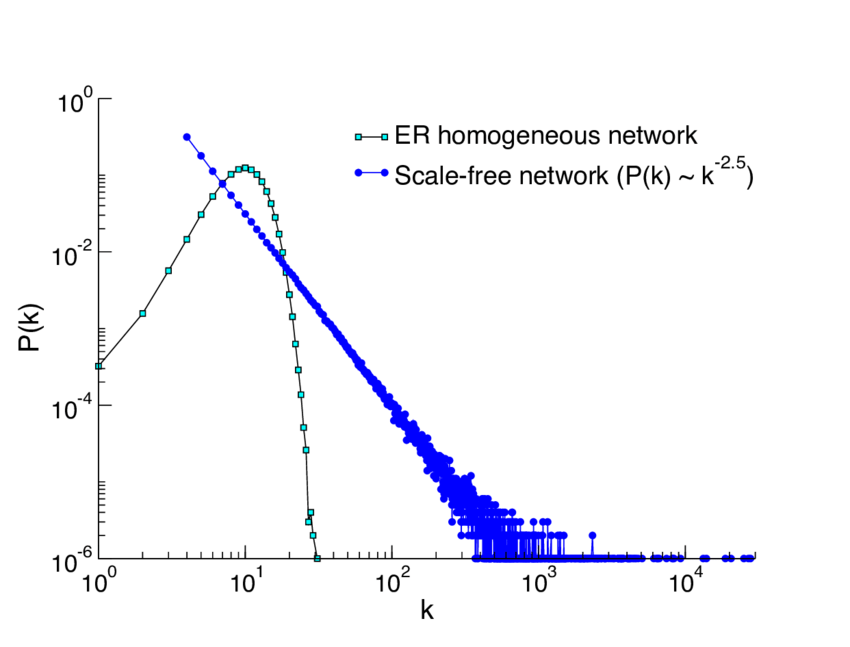
\includegraphics[width=10cm]{figs/intro/nodedegree-dist.png}
    \caption[Distribution of node degree in a generated network]{Distribution of node degree in a generated network (note log scale of the x-axis) \cite{baronchelli_networks_2013}}
    \label{fig:nddist}
\end{figure}
Existing work on stochastic network tomography - primarily from \cite{thoppe_stochastic_2014} \cite{kolar_distributed_2020} - represents networks in a tree-based topology. As noted in \cref{cha:litreview}, the adoption of this technique is common practice when utilizing multi-cast packet transmission for inferential calculations. Such tree-based models, although useful for simplifying tomographic problems, are poor representations of real systems.

\subsubsection*{Traffic Simulation}
\label{sssec:Itrafficsimulation}

The accumulation of all packets sent between each node in the network (referred to as \textit{network traffic} or simply \textit{traffic}) and its simulation is a key aspect of any network model. The traffic within a network is an accumulation of all packets sent from each switch within that network. The traffic at any single router is therefore determined by the number of components adjacent to it, their respective routing tables, and the number of packets forwarded to them. The current model used within the work of \cite{barnes_stochastic_2020} splits traffic simulation into discrete time steps of a uniform length. We adopt their assumption that each time step is a period small enough that only a single packet is handled by each router in each step.\par
Due to this discretization of network traffic, packets (as one would anticipate) do not traverse instantly from sender to receiver, but rather are delayed at various points along their path. We adopt terminology from the authoritative work of \cite{kurose_computer_2013}, and decompose this delay into four classes:
\begin{itemize}
    \item Processing delay
    \item Transmission delay
    \item Propagation delay
    \item Queuing delay
\end{itemize}
Processing delay is the time required for a network component to analyse the requirements of a packet and then take action on those requirements. Transmission delay is the time taken for the link interface of a network component to transmit the physical bits representing the information onto the transmission interface (i.e. fibre, copper, wireless). Propagation delay is the time taken for the signal to traverse the transmission interface from sender to receiver. This is largely dependent on the type of medium and the physical distance between components. Lastly, queuing delay, for the purposes of our work is defined as the delay a packet experiences while waiting in the buffer of a router.\par
In existing models multiple packets may be forwarded to a single router each time step, and each router is only able to perform one forward per time step. Therefore these packets can accumulate in the respective routers’ queues, awaiting forwarding. These router queue lengths are analogous to queuing-delays in real world systems. The work of \cite{barnes_stochastic_2020} considers only the class of queuing delays when dealing with packet delay measurements, where other work on stochastic tomography (\cite{kolar_distributed_2020}, \cite{he_fisher_2015}) makes no distinction between delay classes, instead dealing only with the generalised concept. As noted in \cite{telchemy_impact_2006}, propagation and processing delays are negligible in realistic applications. We therefore focus primarily on extending the work of \cite{barnes_stochastic_2020} and their focus on queuing delays.\par
Although all packets in a network experience queuing delays, the magnitude of the delay is ultimately dependent on the number of packets within the system at any given point in time; or as it is commonly referred to, the network's \textit{traffic intensity}. Traffic intensity is a result of the number of packets sent over a network by switches.\par
The number of packets a switch sends each time step which has been shown to have a binomial distribution (\cite{barnes_stochastic_2020}) over a set time window. This approaches a Poisson distribution over a large enough number of time steps. From (\cite{barnes_stochastic_2020}), where $n$ denotes the number of time steps, $k$ being the number of packets sent and $s$ being the probability on any given time step that a packet will be sent:
\[\lim_{n\to\infty} \frac{n!}{k!(n-k)!}s^k (1-s)^{n-k} =\frac{s^k e^{-s}}{k!}\]
This known distribution of traffic intensity is key in existing work as it allows for the traffic being sent from a node to be represented as a random variable S with a known distribution and a value of one or zero, depending on whether a packet is sent or not.\par
Prior work assuming constant average traffic intensity has shown that queue lengths, and, consequently, queuing delay converge to a steady state over time. Additionally, given a queue length's dependency on the queue length at the previous time step, it has been shown to be a Markov process (\cite{barnes_stochastic_2020}). However, the queue length for each router is a consequence not only of the number of packets sent $S$, but also of the paths these packets take through the network. Therefore, the routing method used by the network must be scrutinised so as to utilize a Markov chain model and thus represent queuing delay as a random variable \gls{qlen}, as shown in \cite{barnes_stochastic_2020}.\par
For network traffic to be stochastic, any routing protocol must be dynamic in nature. If routing tables were fixed, only a single constant path would be taken by a packet between any two nodes. This would result in traffic variations being solely a product of the packet generation rate of switches. Previous work uses an abstract implementation of the distance-vector routing protocol (\cite{perkins_ad_2003}) to achieve this dynamic routing behaviour. This was accomplished using a global controller to compute the shortest distance between any two nodes using Dijkstra's algorithm and broadcasts this information to all components in the network (\cite{barnes_stochastic_2020}). In Barnes's method the weight of an edge represents the number of packets in the queue of the connected router. This representation is valid, as the queue length is analogous to the number of time steps a packet would wait before completing its traversal of that edge.\par
The use of a network-wide controller in this manner is akin to that of Software Defined Networks (SDNs) where routing logic at the link level is dynamically handled by an SDN controller (see \cite{kreutz_software-defined_2015}). Due to most commercial-grade networks not currently employing SDNs and, to the myriad of security concerns surrounding widespread adoption of SDN technology (\cite{wood_scalable_2021}), we highlight the decentralization of this background traffic routing as a key area of work addressed in \cref{sec:Broutingmechanisms}.\par
Additionally, in the work of \cite{barnes_stochastic_2020}, no distinction is made at a routing level between different types of traffic that the router is forwarding. A packet sent by a monitor node that we are able to draw inference from is treated identically to all other packets. As in \cref{sec:Mnetworkprobing}, we adopt the terminology of \cite{he_network_2021} and refer to this as uncontrolled routing (UR). UR is characterised by observable packets sent between monitor nodes following the underlying routing behaviour of the network. However, modern routers are able to make distinctions between different types of packets and so forward them accordingly. Therefore alternate routing of probe packets is feasible under both normal and SDN conditions. Due to our model varying only the routing restriction for probe packets, we use the term \textit{routing} to refer exclusively to the routing of probe packets. We refer to all non-probe traffic as \textit{background traffic}. We introduce alternative forms of routing (originally presented in \cite{he_network_2021}) in \cref{sec:Broutingmechanisms}, as key targets for extension of the existing model.

\subsubsection*{Inferential Calculations}
\label{sssec:Iinferentialcalculations}

In previous models packets are collected at each monitor node throughout the simulation. The cumulative packet delay distribution for each monitor is then computed at the end of the simulation. This calculation of packet delays is trivial. As packets traverse between monitors both the time they are sent from and the time they arrive at monitors is known. However, the path each packet takes through the network is unknown and uncontrollable (due to UR). Due to this, the only method of identifying nefarious routers is to compute expected delay distributions resulting from every possible subset nefarious of routers and compare these to the observed delay distributions.\par
However, the computation of an expected delay distribution is non-trivial as it is dependent on \gls{qlen}, the number of simulated time steps, and the topology of the network. As presented in \cref{ssec:Icurrentmodels}, one solution (from \cite{barnes_stochastic_2020}), utilises a combined agent-based and Markov Chain Monte Carlo (MCMC) approach for calculating these expected delay distributions.\par
The resulting delay distribution is then compared to the observed delay distribution using techniques from signal analysis (presented in \cite{lynn_introduction_2016}). A correlation metric $C$ is computed, where $C(D_x,D_y)=0$ if $D_x$ has an identical distribution to $D_y$. In this comparison both distributions are probability density functions (PDFs) normalised via L2 normalization to yield the Euclidean norm. This method allows for extremely accurate calculation of nefarious nodes compared to conventional methods of link inference tomography.\par
As this correlation is the sole usable method to gain inference, this approach is extremely domain dependant, unable to detect nefarious behaviour if deployed in a network with a single node different from where it was constructed. Additionally, it is prohibitively expensive to infer packet delay metrics by calculating all candidate PDFs for every possible configuration of nefarious routers.\par
The computation of expected delay distributions for each subset of nefarious routers takes on the order of number of router combinations $\mathcal{O}(2^{|R|})$. Previous work in \cite{belloni_computational_2009} has established the complexity of an MCMC algorithm over a large sample space as $\mathcal{O}(d^3 log d)$ where d is the dimensionality of the sample space, or network in our case, which is known to be $\leq 2\cdot \gls{maxdeg} N + 1$ (\cite{erdos_chromatic_1980}). The total complexity of this method is therefore on the order of:
\begin{align}
\label{eq:mcmcbigo}
    \begin{split}
        &\mathcal{O}( (2\cdot \gls{maxdeg} N + 1)^3 \cdot log(2\cdot \gls{maxdeg} N + 1)\cdot 2^{|R|})\\
        &\mathcal{O}(\gls{maxdeg} N ^3 \cdot log \gls{maxdeg} N \cdot 2^{|R|})
    \end{split}
\end{align}\par
However, one drawback noted in the development of this solution was its sensitivity to network hyperparameters, such as traffic flow and queue length. An alternative approach (in \cite{kolar_distributed_2020}) utilizes a distributed scheme to achieve an inferential time complexity of $\mathcal{O}((NPR)^3)$. Data transfer costs and duplicate computations between nodes in this scheme, however, result in the real-world performance being far worse than this theoretical complexity would indicate (\cite{kolar_distributed_2020}).\par
We therefore aim to establish the use of routing techniques other than UR along with new inference techniques of PD tomography to optimize identification of nefarious routers.r\par

\subsection{Developed Model}
\label{ssec:Idevelopedmodels}
As a part of this work, we have developed a network tomographic model within python for bespoke simulation in a constrained environment. The main adaptations over the precious model, covered in \cref{sec:Broutingmechanisms}, are: decentralization of background routing logic, and distinction of probe packets from background traffic. Additionally we implement two optimisations in the model: selection of a minimal set of paths over which to send probe packets, and probabilistic injection of probe packets over each of these paths. We elaborate on these in \cref{sec:Boptimization}.\par
These additions were made to enable packet delay average (PDA) tomography (outlined in \cref{sec:Mnetworkprobing}) to be used in inferential analysis. Finally we highlight minor features, attention to which might better emulate real-world network behaviour. One such feature is the halting of probe injection before the end of the simulation run-time (\cref{sec:Mnetworkprobing}). This halting is intended to represent real-world situations where an administrator would run a network diagnostic for a set amount of time while the network is under load. We refer to this period of actively probing the network as a \textit{measurement interval}.

\section{Core Concepts}
\label{sec:Icoreconcepts}

In this section we describe how network tomography is able to be posed as an inverse problem, and why this is useful. We introduce generalised concepts of stochastic parameter estimation using inverse approaches, namely, Fisher information and optimization techniques. We give a lower-level explanation of how the Fisher information is computed in \cref{cha:background}. Finally we show how these techniques and their results can be applied directly within the context of our work in (\cref{cha:methodology}) to evaluate the efficacy of our approach.

At the most basic level, an inverse problem is one where observations must be used to determine unknown causal factors (\cref{fig:probleminv}, \cite{sadri_effect_2019}).
\begin{figure}[H]
    \centering
    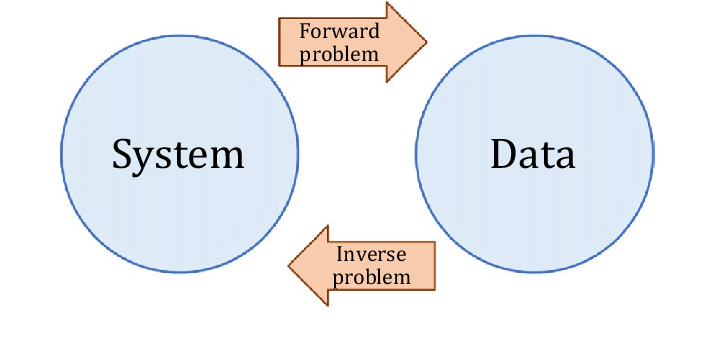
\includegraphics[width=10cm]{figs/intro/inverse_problems.png}
    \caption[Illustration of problem inversion]{Illustration of problem inversion \cite{sadri_effect_2019}}
    \label{fig:probleminv}
\end{figure}
In the context of tomography, packet-level information is observed at monitors and underlying network parameters are calculated; or rather, in the case of stochastic tomography, estimated. Application of network tomography in this manner enables system administrators to monitor for nefarious routers with less traffic overhead and with less system modification, as compared to more conventional methods.\par
As noted in \cref{sec:Imotivationandoutline}, we aim specifically to infer, via observation of packet delay, the presence and location of nefariously delaying routers within a network. We expect the distribution of packet delays, for nefarious nodes, to be more varied and have a heavier tail due to the delaying of packets.\par
To optimize stochastic network tomography, we must consider how to maximise the accuracy of our analysis given the random nature of the network. Intuitively the accuracy of our analysis is limited by the amount of information we are able to collate from our probing. We employ the concept of Fisher information from the field of statistical signal detection (\cite{poor_introduction_1994}) to represent our knowledge of a single element of the network.\par
It follows that the garnered information of all elements in the network can be presented in a Fisher information matrix (FIM) to concretely represent our knowledge of all network elements. As we are primarily measuring the average delay of packets within the network, the FIM represents the information we have about queuing delays of individual routers. This is intrinsically related to the paths we have designated probes to take through that network.\par
In addition to quantifying our knowledge of a network, the FIM has the secondary property of being able to quantify the minimum accuracy of estimations made about the system it represents. This lower bound on the accuracy of inferential estimations is known as the Cramér–Rao bound (CRB). The CRB represents the worst possible inference we can make about a router's queuing delays given collected probing measurements. In \cref{sec:Bparameterestimation} we provide formal definitions of FIM's and their corresponding CRB.We extend on these formal definitions in \cref{sec:Boptimization} to show how the CRB can be improved through optimisations to probe path selection. We additional consider optimisations to the allocation of probes between these paths. To accomplish this, techniques of optimal experiment design (\cite{anthony_c_optimum_1996}) are introduced (in \cref{sec:Boptimization}) and then used (in \cref{sec:Mnetworkprobing}) to maximise inferential accuracy via probe allocation over paths.\par

\section{Summary}
\label{sec:Iintroductionsummary}

In this section we have posed the problem of improving existing network tomography simulations. We noted the utility of approaching this goal as three separate but related problems of: metric inference, information processing, and optimisation. We formally posed an overarching hypothesis that network tomography can be used to estimate routers' buffer queue lengths with sufficient accuracy as to enable inference of packet delaying behaviour by individual routers within real world networks. To better fit our decomposition of the problem, we broke this hypothesis into two independent sub-hypotheses.\par
We introduced previous models of network tomography in stochastic networks, decomposing these models into three sections: network generation, traffic simulation, and inferential calculation. We highlighted the lack of applicability to general topologies and computational intensity of these models as our focus for improvement. 
Optimisation to the code for computational were noted as desirable, as they enable extended simulation run time allowing statistical approximations to converge as noted in Appendix A. The ability to handle general topologies is a key requirement for addressing our hypothesis as it allows for simulation and fair comparison of real world national ISP networks. The final artefact of code is made available at (\cite{sylvester_millar_real_2021}) in hopes that future work will then be able to further expand on this area of work. Specific candidates for future extensions are highlighted in \cref{cha:conc}.